\begin{figure}[H]
	\begin{center}
		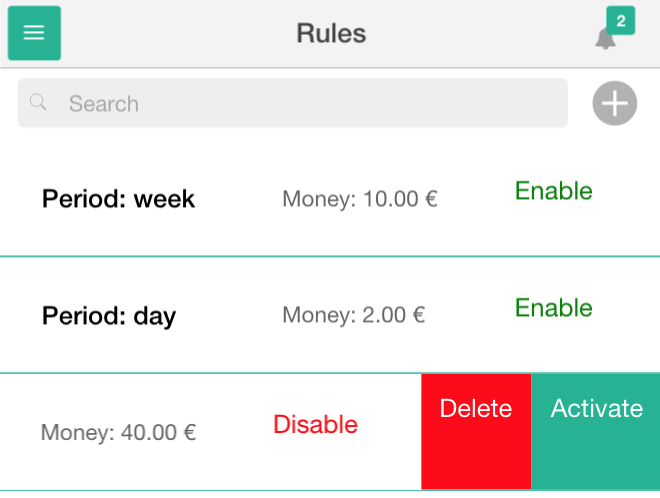
\includegraphics[width=0.5
		\textwidth]{rules/rules.png}
	\end{center}
	\caption{Regras Ativas e Desativas}
	\label{fig:8}
\end{figure}

As regras são constítuidas por periodo (dia, semana e mês), montante máximo que se pode gastar no periodo escolhido e o estado (ativa ou desativa). O objetivo é ajudar o utilizador a controlar os seus custos. Os pagamentos são autorizados apenas se cumprirem as regras e podem ser criadas pelo utilizador ou pelos pais com o objetivo de controlar os pagamentos dos filhos. As regras apenas podem ser eliminadas ou alteradas pelos pais ou pelos filhos caso estes a tenham criadas (ver Figura \ref{fig:8}).

\begin{figure}[H]
	\begin{center}
		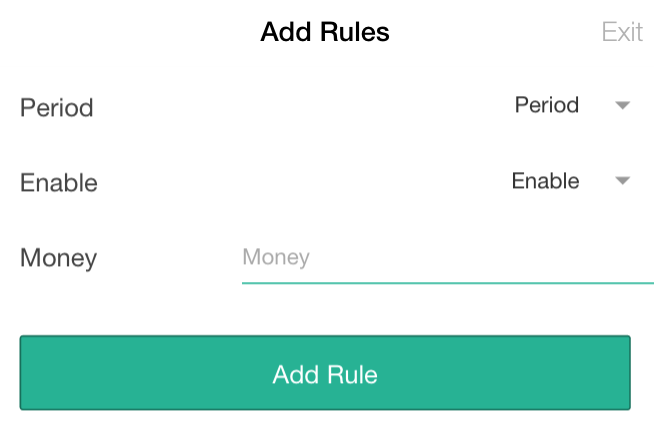
\includegraphics[width=0.5
		\textwidth]{rules/addRule.png}
	\end{center}
	\caption{Adicionar Regra}
	\label{fig:8_1}
\end{figure}

Para adicionar uma nova regra clica-se no botão de adcionar e preenche-se os dados do formulário apresentado na Figura \ref{fig:8_1}.